\documentclass[10pt, a4paper]{article}

\usepackage[frenchb]{babel}
\usepackage[T1]{fontenc}
\usepackage[left=2.2cm, right=2.2cm, top=2.5cm, bottom=2.5cm]{geometry} % Mise en page
\usepackage{tikz}
\usepackage{lscape}
\usepackage{graphicx}

\author{Florian \bsc{Thuin} (06561100) \and Gregory \bsc{Vander Schueren}}
\title{LINGI1131 - Oz Project Report}
\date{\today}

\begin{document}

\maketitle

\section{Data structures}

We use the following 4 main data structures (implemented with records) across the project:

\begin{description}
  \item [GameState:] Top level data structure that holds all the information describing the current state of the game. It is passed around by the gameLoop and modified at each turn. It holds the following information: turn(number), player, trainers(list) and map\_info.
  \item [MapInfo:] Holds the map record and various information like: victory\_position, hospital\_position and width/height for convenience.
  \item [Player:] Describes any player: the actual player, the enemy trainers and the \og{}wild pokemoz\fg{} trainer. It hold the following info: name, image, position, selected\_pokemoz and pokemoz\_list.
  \item [Pokemoz:] Describes any pokemoz: name, type, level, health and xp.

\end{description}

\section{Components}

We divided our code into 5 layers and 12 \og{}components\fg{} (functors). This sections describes the role of each of those components and briefly explains how they interact together:

\begin{description}
  \item[Game logic modules] \hfill
    \begin{description}
     \item \underline{Game:} Main program which is run when you start the game. Its main responsibilities are: getting the program parameters, setting up the main window and receiving keyboard inputs, setting up the intial game state, launching and managing the gameloop. Aside from that it mostly relies on the other components to do all the heavy lifting.
     \item \underline{Fight:} Holds the logic for fights between trainers or with a wild pokemoz. It calls the ShowPlayer method of the interface module after every attack to display the changing pokemoz state.
     \item \underline{AutoPilot:} Manage the automatic play if this option is given in command line. It exposes only one function (GenerateNextInstruction) to the game component.
    \end{description}
  \item[UI modules] \hfill
    \begin{description}
     \item \underline{GameIntro:} Responsible for drawing and managing an interface that allows the player to enter his name and choose his starting pokemoz. It exposes only one function (GetUserChoice) to the game component.
     \item \underline{Map:} Responsible for drawing and managing the map section of the interface. It exposes multiple functions to set items positions and animates items (ie. DrawPlayer or MovePlayer).
     \item \underline{Interface:} Responsible for drawing and managing the lower interface. It exposes multiples functions for displaying the game state (ie. UpdatePlayer1) or getting user input (ie. AskQuestion).
    \end{description}
  \item[State mutators modules] \hfill
    \begin{description}
     \item \underline{GameState:} Helpers to mutate and read data from a gameState record.
     \item \underline{Player:} Helpers to mutate and read data from a player record.
     \item \underline{Pokemoz:} Helpers to mutate and read data from a pokemoz record.
    \end{description}
  \item[Data/assets modules] \hfill
    \begin{description}
     \item \underline{Characters:} Define the game characters (all the pokemoz and trainers).
     \item \underline{Strings:} Define all the text strings displayed in the multiple interfaces.
    \end{description}
  \item[Lib module] Exposes general purpose functions.
\end{description}


%\begin{landscape}

\begin{figure}[!ht]

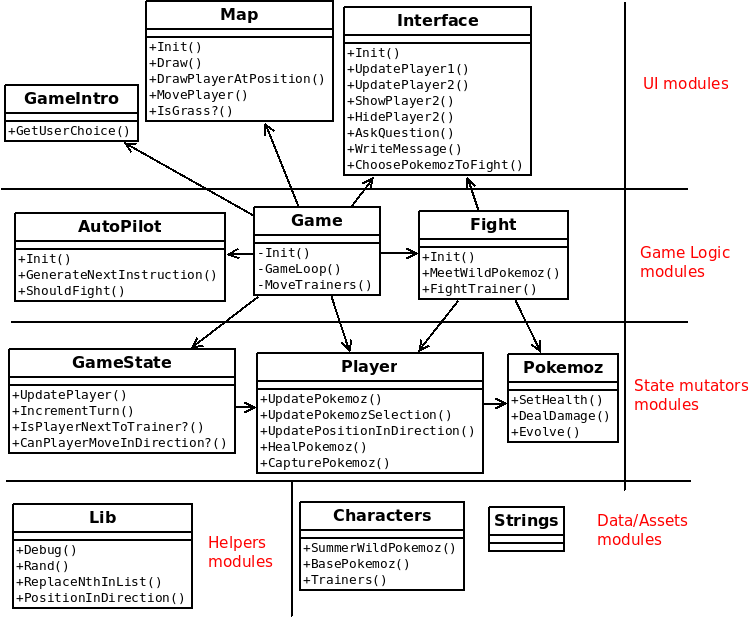
\includegraphics[width=\linewidth]{Diagramme1.png}
\caption{Component diagram of our project}
\end{figure}

%\end{landscape}

\bigskip

\section{State diagrams}

\begin{figure}[!ht]
 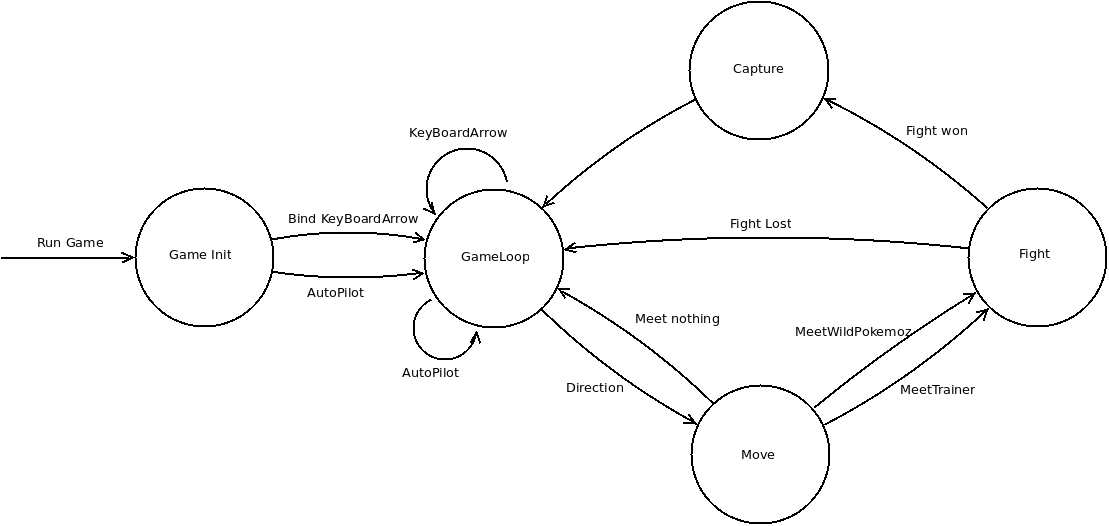
\includegraphics[width=\linewidth]{State_diagram_oz.png}
 \caption{State diagram of our project}
\end{figure}


\end{document}
